\chapter{First chapter in this}%\label{chap:...}
Chapter description

\section{Improving Build Times}

To identify in which parts of the build process to make faster, we measure the time different parts of the Launcher project take. The Launcher project is the main application which depends on many other subprojects. The timings are measured on the Jenkins server and shown in \figureref{fig:launcher_build_times}. The shows the build timings of the Launcher application and the different subprojects (\emph{Oasis-lib, Giraf-Component, Local-db, Barcode-scanner, and Metadata}), as well as the startup time for the emulator.\todo{Kan vi regne med, at submoduler bliver binære filer?}

% Chapters
%\input{part_spring1/somefile}
\begin{figure}
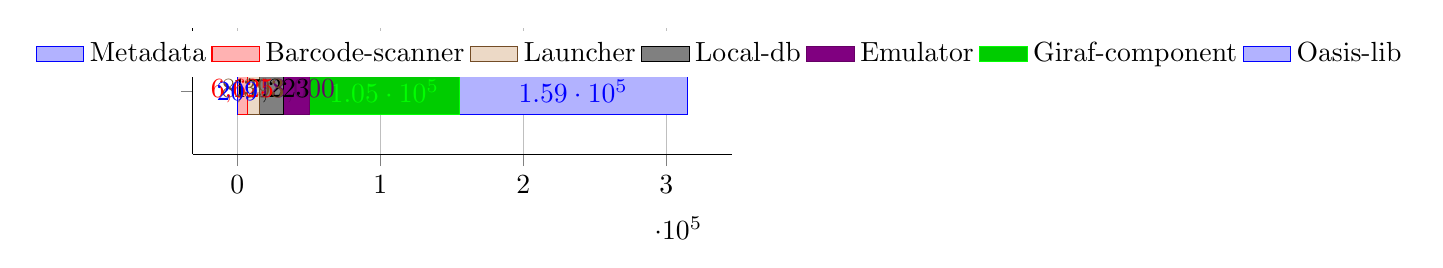
\begin{tikzpicture}
  \begin{axis}[xbar stacked,
axis y line*= none, axis x line*= bottom,
xmajorgrids = true,
ytick = data,
yticklabels = {},
tick align = outside,
xtick pos = left,
bar width=6mm,
y=8mm,
nodes near coords,
legend style={
  legend columns=-1,
  anchor=north,
  draw=none,
},
area legend,]
    \addplot coordinates
    {(209,0)};
    \addlegendentry{Metadata}
    \addplot coordinates
    {(6625,0)};
    \addlegendentry{Barcode-scanner}
    \addplot coordinates
    {(8393,0)};
    \addlegendentry{Launcher}
    \addplot coordinates
    {(17223,0)};
    \addlegendentry{Local-db}
    \addplot coordinates
    {(18000,0)};
    \addlegendentry{Emulator}
    \addplot coordinates
    {(104696,0)};
    \addlegendentry{Giraf-component}
    \addplot coordinates
    {(159497,0)};
    \addlegendentry{Oasis-lib}
  \end{axis}
\end{tikzpicture}
\caption{Timings during build of the Launcher project.}\label{fig:launcher_build_times}
\end{figure}